% Metódy inžinierskej práce

\documentclass[10pt,oneside,english,a4paper]{article}

\usepackage[english]{babel}

\usepackage[IL2]{fontenc} 
\usepackage[utf8]{inputenc}
\usepackage{graphicx}
\usepackage{url} 
\usepackage{hyperref} 

\usepackage{cite}

\usepackage{graphicx}
\usepackage{subcaption}
\usepackage[T1]{fontenc}
\usepackage{lmodern}




\title{Exploring Virtualization Efficiency, Security Enhancements, and Scripting for File and Operating Systems\thanks{CM2134 Assesment}}

\author{Matus ILLITH\\[2pt]
	{\small \texttt{Student ID: 2325478}}\\
	{\small Robert Gordon University Aberdeen}\\
	{\small School of Computing, Engineering and Technology}\\
	{\small \texttt{m.illith@rgu.ac.uk}}
	}

\date{\small 02.10.2024} 


\begin{document}

\maketitle

\begin{abstract}
\ldots
The gaming industry is one of the fastest-growing markets in the world. With rapid improvement in game development, there is no doubt that the computing power requirement keeps rising. With that comes new growing energy expenses. Virtualization and performance have been in the eyes of researchers for years. This paper dives into the cost, energy efficiency and security of virtualizations for ACME Games. This includes examples of File Scripting and Operating System Scripting with adherence to proper coding ethics and security.

\end{abstract}
\newpage
\tableofcontents
\newpage

\section{Virtualisation Efficiency Benefits}
\subsection{Understanding virtualization}
Virtualization in simple terms is the sharing of physical resources between multiple virtual machines. You can think of it as a "computer within a computer, implemented in software."\cite{2.zdroj} This is done by creating an abstraction layer over the physical hardware of the host machine so multiple computers (Virtual Machines) can run on one hardware. They can also share resources such as network cards, CPU, memory, Physical storage and others. Virtual machine is a virtual depiction of machine hardware which is maintained by a virtual machine monitor (VMware Fusion, Oracle VM VirtualBox). (Abstraction diagram here[create/find on internet])The concept of virtualization isn't new it has been here since 1960. But with the introduction of X86 Architecture and platforms, it now has been in the sighs of many companies because it provided simple seamless implementation without significant interruption to operations and low acquisition. 
\cite{1.zdroj}\cite{2.zdroj}

\subsection{Benefits of Virtualization}
The benefits of virtualization are considerable. Virtualization can help with security, scalability, cost cutting, efficient uses of resources and other.
Non virtualized systems can be inefficient when non virtulzed resources aren't in use and the hardware is sitting idle without any computing task ready to run. While in virtulized system once resources become available hypervisor can allocate them accordingly to another task so the physical resources are always in use. With this comes another benefit of security and corruption prevention where in a normal non virtulized system the security and backup lay on one specific machine and user. The virtualized system security depends on the security of the whole system. This can lead to better and more secure disaster prevention where we can back up each VM, so in case of a natural disaster, there isn't any loss of data. In simple terms, virtualization helps with the growth scaleability of an organization.


 For ACME Games virtualization will not only help with cost cutting and security but also with:
\begin{enumerate}
	\item Minimize Servers 
	\item Reduce Hardware
	\item Quick Redeployment
	\item Simpler Backups 
	\item Better Testing
\end{enumerate}

\cite{2.zdroj}\cite{3.zdroj}
\subsection{Cost of virtualization and energy efficiency}
This part delves into total cost of ownership for virtulized systems compared to standard systems and energy efficiency of medium to large organizations. We will look in to direct and indirect costs of virtualization for organizations. With real life examples of companies that went through restructuring of their servers to implement virtualization. 
\subsubsection{Cost of virtualization}
First we need to define what are the major direct cost categories for organization to implement virtulized system.
\begin{enumerate}
	\item Hardware cost

	Represented as expenses that are expected to be bought so virtualization can be implemented to the system. These include physical technologies that would allow to create new virtulized system \cite{2.zdroj}
	\item Software cost

	Are expenses derived from buying and/or licensing software which allows access to virtual machines and all its  possible functions. \cite{2.zdroj}
	\item Deployment costs
 
	These costs are other expenses not directly associated with the concept of virtualization. Costs like disruption to existing operations 
and space improvement.
\end{enumerate}
These are direct costs of implementing virtualization they can be one-time or recurring. These expenses represent the general figure for medium to large firms. These can be cut down further with the right licensing agreement and the right negotiation with hardware providers.

There are also second indirect costs for virtualization
\begin{enumerate}
	\item Training personnel cost
	\item Maintenance cost
	\item Energy cost
\end{enumerate}
\paragraph{Hardware cost}


The initial virtualization cost can be considered high when a classical system is already in place and working. Let's consider the Hardware cost of implementing new servers. We will look into the 2 most popular servers Which are Dell's PowerEdge R6625 and PowerEdge R7625. With these 2 servers, Dell allows extensive customization to get the best price for the best performance and energy efficiency for specific tasks. The table below shows the specifications of each server and the lowest configuration cost per 1 server.
\begin{figure} [h!]
  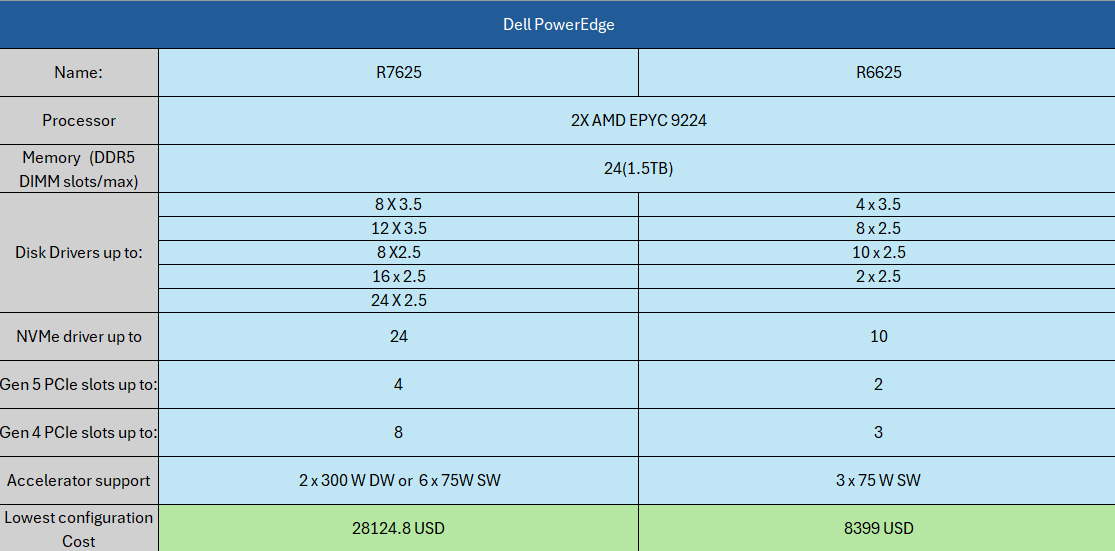
\includegraphics[scale=0.5]{ServerCost.png}
  \caption{Table comparesen made by author. Sourced: \cite{4.zdroj}\cite{5.zdroj}\cite{6.zdroj}}
  \label{fig:rbs.1}
\end{figure}

\newpage
\paragraph{Software cost}


There are multiple virtualization software to consider. We will look into 2  different virtualization software VMware vSphere and Citrix XenServer. 
\begin{enumerate}
	\item VMware vSphere

Offers 2 different options vSphere standard and Foundation.


 vSphere Foundation is their flagship virtualization software which allows access to the full set of virtualization features. This software is for medium to large companies. The set price as of February 2024 is 135 USD per CPU Core. 

For one of the above-mentioned server, it would come to 7200 USD Yearly

vSphere Standard is aimed at small to medium-sized companies. It offers essential virtualization capabilities.
vSpahere standard is priced at 50 USD per CPU core.

For one of the above-mentioned server, it comes to 2400 USD Yearly 

	\item Citrix XenServer
	
	Also Offers Standard and Premium Edition. Unlike vSphere, XenServer Operates on a cost per-CPU socket.

Their standard edition is entry-level virtualization software for lower cost and organizations can still benefit from Technical Support and Maintenance. Nevertheless, the Premium version offers GPU virtualization, Dynamic Workload Balancing, Thin provisioning for shared block storage devices and other features which are essential to  ACME Games. 

The premium version for 1-4 Sockets is 875 USD per socket per year. 
The standard version price for 1-4 sockets is 440 USD per socket per year. 

The price goes down when more sockets are licensed.

\end{enumerate}


\subsubsection{Energy efficiency}
The cost of Energy is hard to predict due to constant economic changes. The cost of energy changes rapidly each month. However from research done by  Jukka Kommeri, Tapio Niemi and Olli Helin in their Energy Efficiency of Server Virtualization from 2012\cite{1.zdroj} shows that with correct implementation virtualization can save energy. In their words "research indicates that idle power consumption of virtualized server is close to zero" \cite{1.zdroj}.


\paragraph{Real world example}
As research into virtualization progresses even more we can expect that energy consumption will lower. 
Case study done in 2010 by K. Thirupathi Rao,P. Sai Kiran and  L.S.S.Reddy(Energy Efficiency in Datacenters through 
Virtualization: A Case Study \cite{7.zdroj}) indicetes that after virtualization datacenter obtained power improvement of 65 percent furthermore data center reduced their number of servers from 500 to 140. Practical investigation in to Croatian company done in 2012 that went through virtualization is the best example for ACME Games. They used Dell PowerEdge 2970 servers for their virtualization. Figure 2 shows lower numbers of servers with predicted growth of 0.25 server per year.\cite{2.zdroj}
\begin{figure} [h!]
  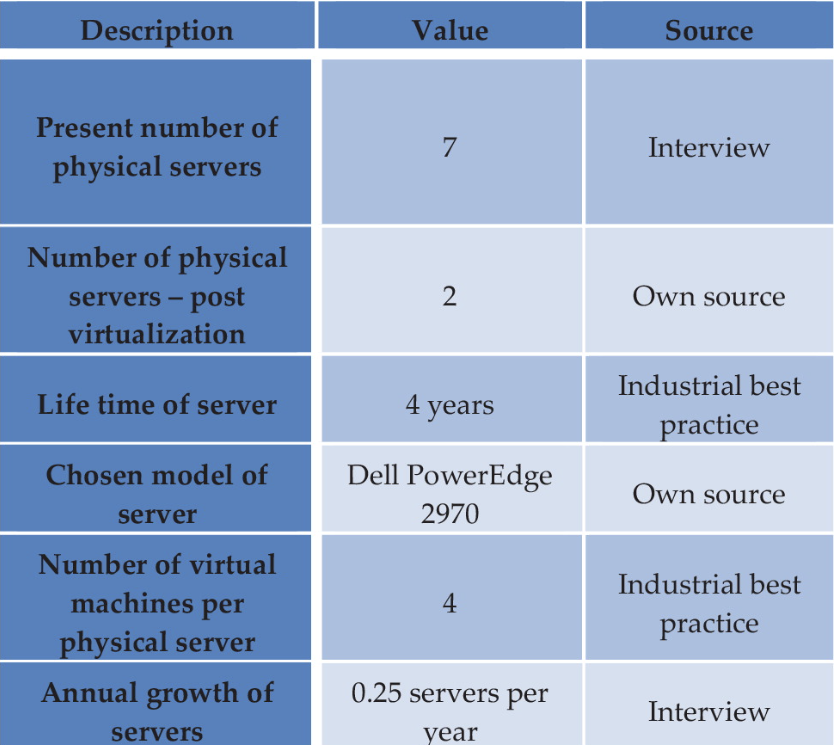
\includegraphics[scale=0.7]{CroatiaTableTechnical.png}
  \caption{Table from: \cite{2.zdroj}}
  \label{fig:rbs.1}
\end{figure}
\newpage
Their virtualized system yields economic energy efficiency of 72.41 percent. The energy cost of their non-virtualized system per year was 45,439.69 USD(adjusted to inflation as of 2024) while their virtualized system 12,535.19 USD (Adjusted to inflation as of 2024). This is 27.59 percent less energy consumed per year.

Overall the economic effect of virtualization for the company was 57.63 percent.


There it is safe to assume that with a correct implementation of virtualization, ACME Games can save on energy consumption, resources and capital.

\section{Security Issues}
Any technological enterprise's biggest concern is the mitigation of unauthorised access to company data. This unauthorised access can be within the company's corporate hierarchies or a malicious attack by a third party. While access permission within a company's structure is achieved by setting up correct entry dispensation and secured data movement infrastructure within the company's internal systems, third-party attacks are harder to prognosticate, therefore establishing robust threat assessment and a durable security panel is exceedingly important compared to other parts of virtualization.
\subsection{Operating system security issues}
In this day and age, we can find operating systems everywhere. This leads to day-to-day exponential improvement in developing malicious algorithms to infect our Operating system. Multiple common vulnerabilities can be exploited
\begin{enumerate}
	\item Buffer Overflow
	\item Code Injections
	\item Privilege Escalation
	\item Denial of Service
	\item Zero-Day
\end{enumerate}
A great example is Microsoft's vulnerability issue from 2023 which was patched in February 2024 and tracked under code CVE-2024-21338. This issue affected the kernel mode in different versions of windows 10 and 11. This exploit used CWE-822 Weaknes where attacker supsedies internal pointer for memory location which wasn't expected. If the pointer dereference in to write the attacker can start modification of variables or carry out code execution.On the other hand direfferencing pointer to read allows reading of sensitive data. This issue fall in to Zero-Day exploit.


This part dives into the most common security issues being exploited. 

\subsubsection{Buffer Overflow}
A buffer overflow occurs when more information is written to the buffer beyond its memory. Buffer overflow attack on a system aims to modify the stat of memory so a third party can execute code which would allow them to 
\subsubsection{Code Injections}
\subsubsection{Privilege Escalation}
\subsubsection{Denial of Service}
\subsubsection{Zero-Day}
\subsection{Virtualization security issues}

\begin{enumerate}
	\item 
	\item 
	\item 
\end{enumerate}
\newpage
\section{File System Scripting}
\newpage
\section{Operating System Scripting}
\newpage
\section{Conclusions}
\bibliography{References}
\bibliographystyle{plain} % prípadne alpha, abbrv alebo hociktorý in

\end{document}